\documentclass[11pt,letterpaper,oneside]{amsart}
\usepackage{fancyhdr}
%\usepackage[headings]{fullpage}
\usepackage{graphicx,subfigure}
\usepackage{wrapfig}
\usepackage{amssymb,amsmath,latexsym,wasysym,mathrsfs,amsfonts,amsthm}
\usepackage{multicol}
\usepackage{geometry}
\usepackage{float}
\usepackage{color}
\usepackage{multirow}       %Needed for spanning rows
\usepackage{listings}
\usepackage{algorithmic}
\usepackage{ulem}

\begin{document}

Group 19 --- Michael Andrews and Ian Collier
Project Step 3

\section*{\textsc{url} for draft \textsc{html}}

\sout{www.iancollier.host}

Temporary location: \texttt{http://flip3.engr.oregonstate.edu:8343}

\section*{Outline}

The project will be a simplified and abstracted view of an automotive suppply chain.  The selection of automobiles is arbitrary, and intended simply to make the relationships intuitive for the user.  The basic intent is to have a series of relationships that will allow the user to track parts suppliers, parts requirements, and orders in such a way that they can easily determine at any given time what supplies need to be procured, and at what price, to meet orders.

\section*{Changes for Step 2}

\begin{itemize}

\item Which keys are foreign (and which domestic) has been clarified, both in the Outline and in the Schema.  (Foreign keys in the schema are now indicated by an asterisk.)

\item The Model-Colors relationship has been replaced with a Trimline-Colors relationship, and removed as an entity-in-itself.  This suggestion was made in both TA and peer feedback.  Additionally, because this is a many-to-many relationship table, that table no longer has its own auto-incrementing key.

\item A suggestion was made in group review to add default values for several attributes which cannot be null.  That suggestion has not been adopted, since the database is (within its own fictional universe) intended to reflect physical realities; a default value for the "Quantity on Hand" attribute of the "Parts" entity, which was one of the suggestions, could result in the database being automatically populated with inaccurate data.  The correct behavior if an attempt is made to add rows without knowing the values for those attributes should be to fail with an error.  Similarly, if a customer attempts to order a car but does not specify either a trimline (which implies a model) or a model (which defaults to a trimline,) they should be told they need to pick something.

\item The \textsc{erd} has been embiggened.

\item The Base Model attribute of Model has had its name changed to Base Trimline rather than making it recursive; the previous name was a typo.

\end{itemize}

\section*{Changes for Step 3 Draft}

\begin{itemize}

\item Key and table names have been changed to lower case, underscore separated.  Keys named 'key' have been changed to 'id' because MariaDB considers key a reserved word.

\item Both attributes in model{\textunderscore}colors have had on delete cascade added to them.

\item Trimline's default model now cascades on deletion.

\item Trimline's default color now cascades to null on deletion.

\end{itemize}

\section*{Review Feedback on Step 3 Draft}

Only one peer review had specific questions and changes; it's included below:

\begin{itemize}

\item "Your DDL file looks good. I was able to successfully import it into phpmyadmin with no errors or issues. I imported again after tables had been created and your drop table if exists statements also look good! Also the samples data was successfully inserted into the tables.

"Looking at your HTML I see on your "Body" page that you have a search field. I know it is still early so you will probably make changes, but maybe specify what can be searched there. Only models? You could also throw and update table header and delete table header in your html table.

"What will the "save changes" buttons do? Will that be a type of 'update' function? If I decide to change trimline and color on the drop downs on the Order page, will hitting save changes update it? Will it update only the ones that I have changed they drop down values or specific ones?

"One question I have is about colors. The color name is the primary key but how are you handling potential duplicate colors being entered into the table?

"I don't have any comments on your query file, everything looks good to me. You have all the insert, delete, and update statements needed as well as some really good query statements that I think will work really well with your database. Good job!

With regard to colors, duplicates are not an issue.  Because a primary key needs to be unique, duplicates cannot be entered, and that's intended behavior.  A duplicate color would serve no purpose.

With regard to what the update and save functions do, the intended behavior will be for update to populate a form with the fields of the item, and for save to commit the item back to the database, incorporating any (legal) changes that might have been made.  (The auto-incrementing keys will be reported, but will not be alterable.)

With regard to the search behavior, a new page has been added with checkboxes to allow for searching any or all of Models, Trimlines, Orders, and Parts by name.

\end{itemize}

\section{Changes for Step 3 Final}

Dedicated search page added; queries added to support its behavior.

\section*{Entities}

We will have the following entities:

\subsection*{models}
The model represents a basic car model.  The intrinsic attributes it needs are:
\begin{itemize}
	\item \emph{id (Primary Key)}
	
	This should be an autoincrementing integer.
	
	\item \emph{name}
	
	Each Model type needs name; this should be a 255 character max string.  It must not be the same as the name of any other Model, or of any Trimline.  It cannot be null.
	
	\item \emph{base{\textunderscore}trimline (Foreign Key)}
	
	Each Model must have a Trimline designated as its base version; this field cannot be null and must contain the key of a Trimline which exists in the database.  Consequently, this field will be an integer.
	
	
\end{itemize}

The other properties of cars will be simulated through relationships with other entities.

\subsection*{trimlines}

\begin{itemize}
	\item \emph{id (Primary Key)}
	
	Each Trimline needs a key; this can be an autoincrementing integer. Cannot be null.
	
	\item \emph{name}
	
	Each Trimeline needs a name; this should be 255 character max string, and must not be the same as the name of any Model or any other Trimline.  Cannot be null.

	\item \emph{model (Foreign Key)}
	
	Each Trimline must have exactly one Model associated with it; this field will store the key of that Model.  It cannot be null.  This should cascade on deletion.
	
	\item \emph{default{\textunderscore}color (Foreign Key)}
	
	Each Trimline needs a default color.  30 character-max string, must be the key of a Color.  Should cascade to null.

\end{itemize}

\subsection*{colors}

\begin{itemize}
	\item \emph	{name (Primary Key)}
		Each color must have a unique name.  This should be a string, thirty characters maximum, must be unique, and cannot be null.  This can also serve as the key.
		
\end{itemize}

\subsection*{parts}

The part entity represents components, by SKU.

\begin{itemize}

\item \emph{id (Primary Key)}

	This should be an auto-incrementing integer.
	
\item \emph{name}

	This should be a 255 character string field, which does not need to be unique.
	
\item \emph{quantity{\textunderscore}on{\textunderscore}hand}

	This should be an integer, and should never be null.
	
\item \emph{cost}

	This should be an integer, and can be null. (If a part has become unavailable.)
	
\end{itemize}

\subsection*{part{\textunderscore}requirements}

This entity will hold tuples indicating how many of each type of part a given model or trimline requires.  (A specific trimline may require additional parts that the underlying model does not; for example, a luxury model might require a fancy GPS while the base model gets an Etch-a-Sketch and a road atlas from \oldstylenums{1962}.)

\begin{itemize}

\item \emph{id (Primary Key)}
	This should be an autoincrementing integer.
	
\item \emph{associated{\textunderscore}model (Foreign Key)}
	This should be the key of the Model to which the tuple applies.  Integer, can be null if and only if Associated Trimline is not null, must exist in DB if not null.
	
\item \emph{associated{\textunderscore}trimline (Foreign Key)}
	This should be the key of the Trimline to which the tuple applies.  Integer, can be null if and only if Associated Model is not null, must exist in DB if not null.
	
\item \emph{associated{\textunderscore}part (Foreign Key)}

	This should be the key of the part with which the tuple is associated.  Integer, cannot be null, must exist in DB.
	
\item \emph{quantity}

	This should be the quantity of the part needed for the pairing; must be an integer, must be at least one, cannot be null.

	
\end{itemize}

\subsection*{orders}

This represents an actual order for a vehicle.  We'll abstract the customer details to just a name; the jerks can come pick it up at the factory.

\begin{itemize}

\item \emph{id}
	This should be an autoincrementing integer; it will represent the order number, so maybe we'll start it off at like 5 million so it looks like we're more successful than we are.

\item \emph{customer}

	The name of the customer; 255 character string, cannot be null, does not need to be unique.
	
\item \emph{trimline (Foreign Key)}
	
	The key of a Trimline; cannot be null and must exist in the database.
	
\item \emph{color (Foreign Key)}

	The color desired by the customer.  Thirty character string, cannot be null, must be the key of a Color which has a row in ModelColors corresponding to the Model corresponding to the desired Trimline.  (e.g., the customer wants a Trimline called a Thuggee in Blue.  The Thuggee is a trimline of Dacoity; ModelColors does not have a row for the Dacoity in Blue.  The order is invalid.)
	
\end{itemize}

This is already complicated enough, so we won't worry about when the customer wants it by.  The jerks can come by the factory every day until we have something for them.  Our motto is, "The Customer is Always a Sap."

\section*{Relationships}

\subsection*{Models have Trimlines}

Each model must have at least one Trimline, and can have as many as needed.  Each Trimline is associated with one and only one Model. This is a one-to-many relationship.

\subsection*{Models have Colors}

Each model must be available in at least one color, but can be available in as many as needed.  This is a many-to-many relationship.

\subsection*{Models need Parts}

Each Model needs at least one instance of one part, but may need an arbitrary quantity of an arbitrary number of parts.  Any given part can be needed by any number of models, but can be needed by none.  This is a many-to-many relationship.

\subsection*{Trimlines need Parts}

Each Trimline may need any quantity of any number of parts, but can require none.  The parts needed can overlap with those required with the underlying Model of the Trimline.  Parts need not be needed by Trimlines, but can be needed by any number of them.  This is a many-to-many relationship. 

\subsection*{Orders need Trimlines}

Each order must have exactly one Trimline specified.  Any number of orders can specify the same Trimeline.  This is a many-to-one relationship.

\subsection*{Orders need Colors}

Each order must specify a Color which must be available for the Model associated with the Trimline specified in the order.  An order which specifies an invalid combination should be rejected.  A Color, of course, may be associated with any number of orders.  This is a many-to-one relationship.

\section*{Entity Relationship Diagram}

\begin{figure}[H]
	\centerline{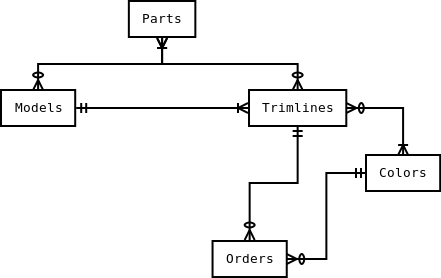
\includegraphics[scale=1.2]{erddraft.png}}
\end{figure}

\section*{Schema}

\begin{figure}[H]
	\centerline{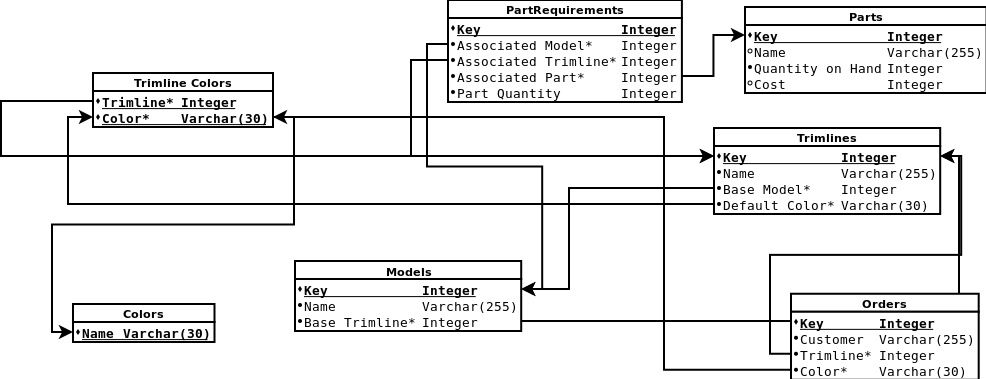
\includegraphics[scale=.55]{schema.png}}
\end{figure}


\end{document}